\documentclass[10pt]{article}
\usepackage[margin=0.8in]{geometry}
\usepackage{amsmath,amssymb,booktabs,array,tabularx,xcolor,enumitem,caption}
\usepackage{listings}
\usepackage{xurl}
\usepackage{hyperref}
\usepackage{tikz}
\usetikzlibrary{positioning,arrows.meta,calc}
\hypersetup{colorlinks=true,linkcolor=blue!50!black,urlcolor=blue!50!black}
\setlist{itemsep=1pt,topsep=3pt}
\definecolor{inp}{HTML}{EDEDEA}
\definecolor{feat}{HTML}{E6F1E0}
\definecolor{enc}{HTML}{DCE8F7}
\definecolor{lat}{HTML}{E4DDF4}
\definecolor{dec}{HTML}{FBE3D6}
\definecolor{ink}{HTML}{333333}
\definecolor{badge}{HTML}{B03A2E}
\definecolor{codebg}{HTML}{F7F7F5}
\lstset{language=Python, basicstyle=\ttfamily\scriptsize, backgroundcolor=\color{codebg}, frame=single,
  rulecolor=\color{ink!25}, breaklines=true, breakatwhitespace=false, columns=fullflexible, keepspaces=true,
  showstringspaces=false, keywordstyle=\color{blue!55!black}, commentstyle=\color{green!35!black}\itshape,
  stringstyle=\color{red!45!black}, upquote=true, aboveskip=6pt, belowskip=6pt, xleftmargin=2pt, xrightmargin=2pt}
\newcommand{\code}[1]{{\small\path{#1}}}
\newcommand{\shape}[1]{{\small\ttfamily [#1]}}
\DeclareRobustCommand{\vb}[1]{\tikz[baseline=-0.6ex]\node[circle, fill=badge, text=white, font=\sffamily\bfseries\scriptsize, inner sep=1pt, minimum size=3.6mm]{#1};}
\newcolumntype{L}[1]{>{\raggedright\arraybackslash}p{#1}}

\title{STARS multi-agent forecaster and crowd simulator\\[2pt] \large inputs, featurization, model, variants and their losses}
\author{Code: \href{@@REPO@@/tree/@@COMMIT@@}{\texttt{michaelmunje/stars\_steps\_extension} @ \texttt{@@SHORT@@}}}
\date{2026-11-18}

\begin{document}
\maketitle

\noindent\textbf{How to read this.} Section~\ref{sec:overview} is the whole system on one page; red letters
mark the components a variant modifies. Section~\ref{sec:blocks} defines the standard building blocks used.
Section~\ref{sec:features} defines every number the model receives. Section~\ref{sec:core} is the core model and
its training loss. Section~\ref{sec:variants} gives each variant in the same format, including its own loss.
Section~\ref{sec:sim} is the simulator loop. Every code listing is copied verbatim from commit \texttt{@@SHORT@@};
its title links to those exact lines on GitHub.

\tableofcontents

%======================================================================
\section{The system at a glance}\label{sec:overview}
%======================================================================
\textbf{Task.} Input: the last 3.2 s (8 steps of $\Delta t=0.4$ s) of every pedestrian in a scene. Output:
$K$ (here 20) possible futures of 4.8 s (12 steps) for \emph{all} pedestrians at once, an array
\shape{K, N, 12, 2}: sample $k$ is one complete future of the scene, $N$ is the number of pedestrians and
the last axis is $(x,y)$ in metres.

\begin{figure}[h!]
\centering
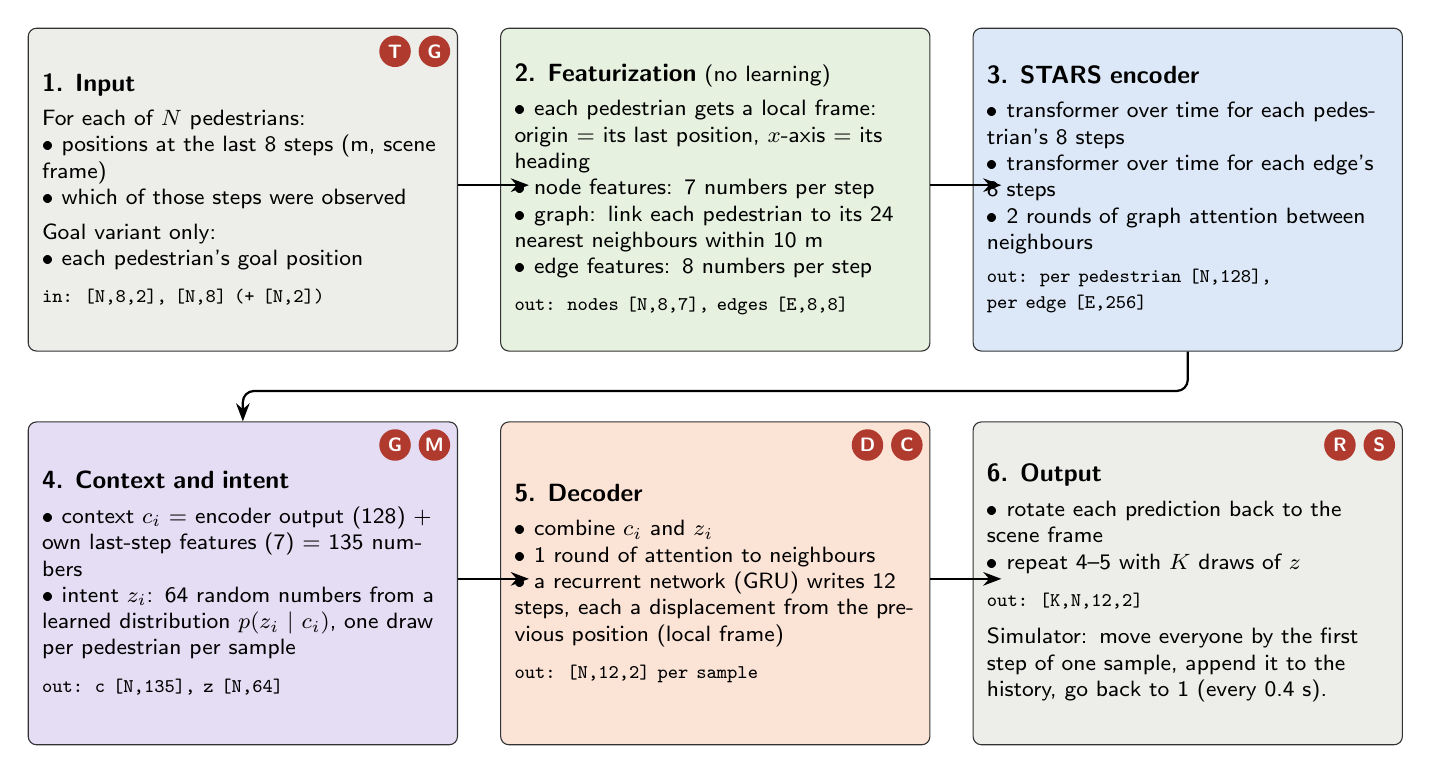
\begin{tikzpicture}[font=\sffamily\footnotesize, >={Stealth[length=2.3mm]},
  box/.style={draw=ink, rounded corners=3pt, align=left, text width=51mm, minimum height=41mm, inner sep=5pt, anchor=north west},
  b/.style={circle, fill=badge, text=white, font=\sffamily\bfseries\scriptsize, inner sep=1pt, minimum size=4mm}]
\node[box, fill=inp] (A) at (0,0) {\textbf{\small 1. Input}\\[3pt]
  For each of $N$ pedestrians:\\
  \textbullet\ positions at the last 8 steps (m, scene frame)\\
  \textbullet\ which of those steps were observed\\[3pt]
  Goal variant only:\\
  \textbullet\ each pedestrian's goal position\\[4pt]
  {\ttfamily\scriptsize in: [N,8,2], [N,8] (+ [N,2])}};
\node[box, fill=feat] (B) at (6.0,0) {\textbf{\small 2. Featurization} (no learning)\\[3pt]
  \textbullet\ each pedestrian gets a local frame: origin = its last position, $x$-axis = its heading\\
  \textbullet\ node features: 7 numbers per step\\
  \textbullet\ graph: link each pedestrian to its 24 nearest neighbours within 10 m\\
  \textbullet\ edge features: 8 numbers per step\\[4pt]
  {\ttfamily\scriptsize out: nodes [N,8,7], edges [E,8,8]}};
\node[box, fill=enc] (C) at (12.0,0) {\textbf{\small 3. STARS encoder}\\[3pt]
  \textbullet\ transformer over time for each pedestrian's 8 steps\\
  \textbullet\ transformer over time for each edge's 8 steps\\
  \textbullet\ 2 rounds of graph attention between neighbours\\[4pt]
  {\ttfamily\scriptsize out: per pedestrian [N,128],\\ per edge [E,256]}};
\node[box, fill=lat] (D) at (0,-5.0) {\textbf{\small 4. Context and intent}\\[3pt]
  \textbullet\ context $c_i$ = encoder output (128) + own last-step features (7) = 135 numbers\\
  \textbullet\ intent $z_i$: 64 random numbers from a learned distribution $p(z_i\mid c_i)$, one draw per pedestrian per sample\\[4pt]
  {\ttfamily\scriptsize out: c [N,135], z [N,64]}};
\node[box, fill=dec] (E) at (6.0,-5.0) {\textbf{\small 5. Decoder}\\[3pt]
  \textbullet\ combine $c_i$ and $z_i$\\
  \textbullet\ 1 round of attention to neighbours\\
  \textbullet\ a recurrent network (GRU) writes 12 steps, each a displacement from the previous position (local frame)\\[4pt]
  {\ttfamily\scriptsize out: [N,12,2] per sample}};
\node[box, fill=inp] (F) at (12.0,-5.0) {\textbf{\small 6. Output}\\[3pt]
  \textbullet\ rotate each prediction back to the scene frame\\
  \textbullet\ repeat 4--5 with $K$ draws of $z$\\[4pt]
  {\ttfamily\scriptsize out: [K,N,12,2]}\\[4pt]
  Simulator: move everyone by the first step of one sample, append it to the history, go back to 1 (every 0.4 s).};
\draw[->, thick] ($(A.north east)+(0,-2)$) -- ++(0.9,0);
\draw[->, thick] ($(B.north east)+(0,-2)$) -- ++(0.9,0);
\draw[->, thick, rounded corners] (C.south) -- ++(0,-0.5) -| (D.north);
\draw[->, thick] ($(D.north east)+(0,-2)$) -- ++(0.9,0);
\draw[->, thick] ($(E.north east)+(0,-2)$) -- ++(0.9,0);
\node[b] at ($(A.north east)+(-0.3,-0.3)$) {G};
\node[b] at ($(A.north east)+(-0.8,-0.3)$) {T};
\node[b] at ($(D.north east)+(-0.3,-0.3)$) {M};
\node[b] at ($(D.north east)+(-0.8,-0.3)$) {G};
\node[b] at ($(E.north east)+(-0.3,-0.3)$) {C};
\node[b] at ($(E.north east)+(-0.8,-0.3)$) {D};
\node[b] at ($(F.north east)+(-0.3,-0.3)$) {S};
\node[b] at ($(F.north east)+(-0.8,-0.3)$) {R};
\end{tikzpicture}
\caption{The whole system. Red letters mark where each variant changes something (Table~\ref{tab:legend}).}
\label{fig:overview}
\end{figure}

\begin{table}[h!]
\centering\small
\begin{tabularx}{\textwidth}{@{}c L{3.6cm} X c@{}}
\toprule
& Variant & What it changes & Section \\
\midrule
\vb{T} & Training data & which datasets are used; architecture unchanged & \ref{sec:v-data} \\
\vb{G} & Goal-conditioned & adds each pedestrian's goal to the input and context (privileged information) & \ref{sec:v-goal} \\
\vb{M} & Mode & uses the most likely intent instead of a random one (inference only) & \ref{sec:v-mode} \\
\vb{S} & Least-colliding selection (``STARS improved'') & draws more samples, keeps those with the fewest collisions (inference only) & \ref{sec:v-select} \\
\vb{C} & Collision-aware & decoder refinement round + collision penalty in the loss & \ref{sec:v-coll} \\
\vb{D} & Diffusion decoder & replaces the intent and GRU decoder with denoising diffusion & \ref{sec:v-diff} \\
\vb{R} & Rollout fine-tuning & extra training through the simulator loop & \ref{sec:v-rft} \\
\bottomrule
\end{tabularx}
\caption{Variants and where they act.}
\label{tab:legend}
\end{table}

%======================================================================
\section{Building blocks}\label{sec:blocks}
%======================================================================
\begin{description}[leftmargin=0pt, itemsep=3pt]
\item[Temporal transformer.] A standard transformer encoder applied along the time axis of one sequence
(here the 8 observed steps of one pedestrian or one edge), with learned positional encodings; the output at
the last step summarises the sequence.
\item[Graph attention (\texttt{TransformerConv}, PyTorch Geometric).] Each node $j$ updates its vector $h_j$ from
its incoming neighbours $i$ with attention weights that also depend on the edge vector $e_{ij}$:
$h'_j = W_1h_j + \sum_{i}\alpha_{ij}\,(W_2h_i+W_3e_{ij})$, with
$\alpha_{ij}=\operatorname{softmax}_i\big((W_4h_j)^\top(W_5h_i+W_3e_{ij})/\sqrt d\big)$ (multi-head, with a learned gate between
the two terms). We always add it residually and normalise: $h\leftarrow\mathrm{LayerNorm}(h+\mathrm{TransformerConv}(h))$.
\item[GRU.] A gated recurrent unit: a recurrent cell $s_{t}=\mathrm{GRU}(\text{input}_t, s_{t-1})$ used here to write
one step at a time.
\item[CVAE.] A conditional variational autoencoder: the output depends on the input $c$ and a random latent
$z$. A prior network gives $p(z\mid c)$; during training a posterior network $q(z\mid c,y)$ that also sees the
answer $y$ provides $z$, and a KL term keeps $q$ close to $p$, so at test time sampling $z\sim p(z\mid c)$ gives
diverse, plausible outputs.
\end{description}

%======================================================================
\section{Inputs and featurization}\label{sec:features}
%======================================================================
Featurization has no learned parameters. It turns raw positions into numbers that do not depend on where the
scene is or which way it faces.

\begin{figure}[h!]
\centering
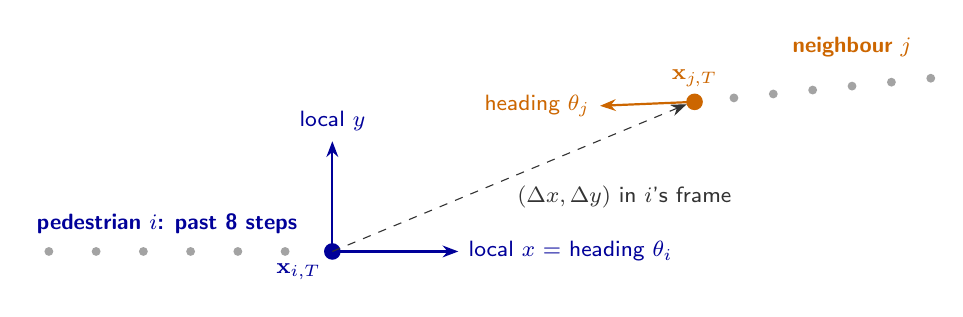
\begin{tikzpicture}[>={Stealth[length=2mm]}, font=\sffamily\footnotesize]
\foreach \x in {-3.6,-3.0,-2.4,-1.8,-1.2,-0.6} \fill[ink!45] (\x,0) circle (1.6pt);
\fill[blue!60!black] (0,0) circle (3pt) node[below left=1pt] {$\mathbf x_{i,T}$};
\draw[->, thick, blue!60!black] (0,0) -- (1.6,0) node[right] {local $x$ = heading $\theta_{i}$};
\draw[->, thick, blue!60!black] (0,0) -- (0,1.4) node[above] {local $y$};
\node[blue!60!black, font=\sffamily\footnotesize\bfseries] at (-2.1,0.35) {pedestrian $i$: past 8 steps};
\foreach \x/\y in {7.6/2.2,7.1/2.15,6.6/2.1,6.1/2.05,5.6/2.0,5.1/1.95} \fill[ink!45] (\x,\y) circle (1.6pt);
\fill[orange!80!black] (4.6,1.9) circle (3pt) node[above=2pt] {$\mathbf x_{j,T}$};
\draw[->, thick, orange!80!black] (4.6,1.9) -- (3.4,1.85) node[left] {heading $\theta_j$};
\node[orange!80!black, font=\sffamily\footnotesize\bfseries] at (6.6,2.6) {neighbour $j$};
\draw[->, dashed, ink] (0,0) -- (4.5,1.87) node[midway, below right=-1pt] {$(\Delta x,\Delta y)$ in $i$'s frame};
\end{tikzpicture}
\caption{Local frame of pedestrian $i$ and the edge between $i$ and a neighbour $j$.}
\label{fig:frames}
\end{figure}

\paragraph{Heading.} $\theta_{i,t}$ is the direction of the last non-zero displacement up to step $t$; before a
pedestrian first moves it takes the direction of that first movement; a pedestrian that never moves has $\theta=0$.

\paragraph{Node features} (7 per step). With $R(\alpha)$ the rotation by $\alpha$, the position of $i$ in its
current frame is $\mathbf p_{i,t}=R(-\theta_{i,T})(\mathbf x_{i,t}-\mathbf x_{i,T})$:

\begin{center}\small
\begin{tabular}{@{}cll@{}}
\toprule
\# & Feature & Formula \\
\midrule
1--2 & position in own frame & $\mathbf p_{i,t}$ (so $(0,0)$ at the last step) \\
3--4 & velocity in own frame & $(\mathbf p_{i,t}-\mathbf p_{i,t-1})/\Delta t$ (0 at $t=1$) \\
5 & speed & norm of features 3--4 \\
6--7 & heading change & $\cos(\theta_{i,t}-\theta_{i,T}),\ \sin(\theta_{i,t}-\theta_{i,T})$ \\
\bottomrule
\end{tabular}
\end{center}

%%SNIP src/baselines/stars_ma_graph.py 105 115 Node features and local frame%%

\paragraph{Graph.} Nodes are the pedestrians visible at the last observed step. Each pedestrian $j$ gets
directed edges $i\to j$ from its 24 nearest pedestrians within 10 m (distances at the last step); information
flows along the edge into $j$.

%%SNIP src/baselines/stars_ma_graph.py 136 162 Neighbour edges%%

\paragraph{Edge features} (8 per step). For edge $i\to j$ at step $t$, in $i$'s frame at that step:

\begin{center}\small
\begin{tabular}{@{}cll@{}}
\toprule
\# & Feature & Formula \\
\midrule
1--2 & where $j$ is, seen from $i$ & $R(-\theta_{i,t})(\mathbf x_{j,t}-\mathbf x_{i,t})$ \\
3--4 & $j$'s heading relative to $i$'s & $\cos(\theta_{j,t}-\theta_{i,t}),\ \sin(\theta_{j,t}-\theta_{i,t})$ \\
5--8 & change of features 1--4 since the previous step & (0 at $t=1$) \\
\bottomrule
\end{tabular}
\end{center}

%%SNIP src/baselines/stars_ma_graph.py 117 134 Edge features%%

%%SNIP src/baselines/stars_ma_graph.py 164 194 Graph construction (all featurization)%%

\subsection*{Worked example: two pedestrians approaching each other}
Alice walks east at 1.2 m/s and is now at $(0,0)$; Bob walks west at 1.0 m/s and is now at $(6.0,0.3)$.
\begin{itemize}
\item \textbf{Input} \shape{2,8,2}: Alice $(-3.36,0),(-2.88,0),\dots,(0,0)$ (0.48 m per step); Bob
$(8.8,0.3),\dots,(6.0,0.3)$ (0.40 m per step).
\item \textbf{Frames}: Alice origin $(0,0)$, heading $0$; Bob origin $(6.0,0.3)$, heading $\pi$ (facing west).
\item \textbf{Node features at the last step}: Alice $(0,0,\ 1.2,0,\ 1.2,\ 1,0)$; Bob $(0,0,\ 1.0,0,\ 1.0,\ 1,0)$:
both at their own origin, moving forward along their own $x$-axis.
\item \textbf{Edge Bob$\to$Alice at the last step}: $(6.0,\ 0.3,\ -1,\ 0,\ -0.88,\ 0,\ 0,\ 0)$: seen from Bob,
Alice is 6 m ahead and 0.3 m to his left, facing him ($\cos=-1$), and the gap shrinks by 0.88 m per step.
\item \textbf{Output} \shape{20,2,12,2}: 20 joint futures. In one sample both drift to their left and pass; in
another both may drift the same way and collide, because each pedestrian's intent is drawn independently
(variants \vb{S} and \vb{C} address this).
\end{itemize}

%======================================================================
\section{Core model}\label{sec:core}
%======================================================================
\subsection{Encoder (upstream STARS, unmodified layers)}
A temporal transformer (2 layers, 4 heads, width 256) reads each node's 8 feature steps and is added to a
node-type embedding; another (3 layers) reads each edge's 8 steps and gives an edge embedding \shape{E,256}.
Two graph-attention rounds mix neighbours, and a linear head gives the representation
$\mu^{\text{enc}}_i\in\mathbb R^{128}$ (the mean head of STARS's own pretraining VAE).

%%SNIP src/baselines/stars_ma_model.py 156 173 Encoder forward pass%%

\subsection{Context and intent}
The context is $c_i=[\mu^{\text{enc}}_i \,\|\, \text{node features of the last step}]\in\mathbb R^{135}$. The prior
$p(z_i\mid c_i)=\mathcal N(\mu_i,\operatorname{diag}\sigma_i^2)$ is an MLP of $c_i$ with $z_i\in\mathbb R^{64}$; the posterior
$q(z_i\mid c_i,\mathbf y_i)$ also reads an MLP encoding of the true future (training only).

%%SNIP src/baselines/stars_ma_model.py 500 516 Context and intent sampling%%

%%SNIP src/baselines/stars_ma_model.py 284 293 Context, prior and posterior networks%%

\subsection{Decoder}
$h_i=\mathrm{GELU}(\mathrm{Linear}([c_i\|z_i]))\in\mathbb R^{512}$; one graph-attention round (with the encoder's
edge embeddings); then a GRU writes 12 displacements, starting from the current velocity $\times\Delta t$. Positions
are their cumulative sum, in the local frame.

%%SNIP src/baselines/stars_ma_model.py 295 307 GRU unroll (12 steps)%%

%%SNIP src/baselines/stars_ma_model.py 323 345 Decoder forward pass (the refine part is variant C)%%

\subsection{Training loss}
With $\mathcal V$ the supervised (pedestrian, future step) pairs, $N_f$ the number of pedestrians with a
supervised future, and $\hat{\mathbf y}_{i,t}$ decoded with a posterior sample $z^q_i=\mu^q_i+\sigma^q_i\odot\epsilon$:
\begin{align*}
\mathcal L_{\text{fc}} &= \frac{1}{|\mathcal V|}\sum_{(i,t)\in\mathcal V}\big\|\hat{\mathbf y}_{i,t}-\mathbf y_{i,t}\big\|_2,\\
\mathcal L_{\text{KL}} &= \frac{1}{N_f}\sum_i \tfrac12\sum_{d=1}^{64}\Big[\log\tfrac{\sigma^{p\,2}_{i,d}}{\sigma^{q\,2}_{i,d}}+\tfrac{\sigma^{q\,2}_{i,d}+(\mu^q_{i,d}-\mu^p_{i,d})^2}{\sigma^{p\,2}_{i,d}}-1\Big],\\
\mathcal L_{\text{core}} &= \mathcal L_{\text{fc}}+\beta\,\mathcal L_{\text{KL}},\qquad \beta=0.0799\ \text{(linearly warmed up over the first 10 epochs)}.
\end{align*}
Optimiser AdamW, learning rate $3\times10^{-4}$ with warm-up and cosine decay, 60 epochs; the checkpoint with the
best validation best-of-20 ADE is kept.

%%SNIP src/baselines/stars_ma_model.py 547 555 Posterior sample and KL%%

%%SNIP src/baselines/train_stars_ma.py 399 403 Masked L2 error%%

%%SNIP src/baselines/train_stars_ma.py 478 482 Total loss (all variants' terms; unused weights are 0)%%

\subsection{Inference}
Encode once, draw $K$ intents per pedestrian from the prior, decode each, rotate back to the scene frame.

%%SNIP src/baselines/stars_ma_model.py 566 579 Inference (oversampling branch is variant S)%%

%======================================================================
\section{Variants}\label{sec:variants}
%======================================================================
Each variant is the core model with only the listed changes.

\subsection{\texorpdfstring{\vb{T}}{[T]} Training data}\label{sec:v-data}
\begin{tabularx}{\textwidth}{@{}L{3.6cm} X L{4.2cm}@{}}
\toprule
Model & Training data & Checkpoint \\
\midrule
STARS (STEPS-only) & STEPS (intent size 32, 16 neighbours) & \code{cvae_kl01_finetune} \\
STARS previous (pooled) & STEPS, PTDPES, Madras, Grand Central, UCY, ETH & \code{cvae_all_lr3e-4_seed42} \\
STARS no ETH/UCY & STEPS, PTDPES, Madras, Grand Central, ATC & \code{cvae_noethucy_nogoal} \\
STARS improved & all 7 incl.\ ATC (3 seeds; seed 2 used) & \code{si_final_base_s2} \\
Protocol A (in progress) & STEPS, PTDPES, Madras, Grand Central only & \code{ep_pre4_s*} \\
Protocol B (in progress) & A, then fine-tuned on 4 ETH/UCY scenes, tested on the 5th & \code{ep_loso_*} \\
\bottomrule
\end{tabularx}

\subsection{\texorpdfstring{\vb{G}}{[G]} Goal-conditioned (privileged)}\label{sec:v-goal}
\begin{description}[leftmargin=2.5cm, style=nextline, itemsep=2pt]
\item[What changes] The model is told where each pedestrian is going.
\item[Extra input] goal features \shape{N,4}: $(\Delta x,\Delta y)$ to the goal in the pedestrian's own frame and the
distance (all divided by 10 m), plus a valid flag. In our benchmarks the goal is the last recorded position of the
track, i.e.\ privileged information.
\item[Architecture] context becomes $[\mu^{\text{enc}}_i\,\|\,\text{last node features}\,\|\,\text{goal}]\in\mathbb R^{139}$ (see the
\texttt{goal} branch of the context listing in Section~\ref{sec:core}).
\item[Loss] unchanged ($\mathcal L_{\text{core}}$).
\item[Checkpoint] \code{cvae_noethucy_goal}; flag \texttt{--goal}.
\end{description}
%%SNIP src/baselines/stars_ma_model.py 73 83 Goal features%%

\subsection{\texorpdfstring{\vb{M}}{[M]} Mode (deterministic)}\label{sec:v-mode}
\begin{description}[leftmargin=2.5cm, style=nextline, itemsep=2pt]
\item[What changes] Use the most likely intent, $z_i=\mu_i$, instead of a random draw; one future per scene.
\item[Architecture / loss] unchanged; works with any CVAE checkpoint (the \texttt{mean=True} branch of
\texttt{sample\_latent} in Section~\ref{sec:core}).
\item[Why] The fair comparison with deterministic baselines such as constant velocity: a random sample from a
spread-out distribution has a larger expected error than its centre.
\end{description}

\subsection{\texorpdfstring{\vb{S}}{[S]} Least-colliding selection (``STARS improved'')}\label{sec:v-select}
\begin{description}[leftmargin=2.5cm, style=nextline, itemsep=2pt]
\item[What changes] At inference, draw $4K$ joint samples and keep the $K$ with the fewest close pairs.
\item[Architecture / loss] unchanged (used with the 7-dataset model of \vb{T}).
\item[Rule] For sample $s$,
\[ C(s)=\sum_{\substack{i<j\\ (i,j)\notin G}}\mathbf 1\Big[\min_t\big\|\hat{\mathbf p}^{(s)}_{i,t}-\hat{\mathbf p}^{(s)}_{j,t}\big\|<0.4\text{ m}\Big]; \]
keep the $K$ samples with the smallest $C(s)$. $G$ are pairs that look like a walking group in the observation
(within 1 m and velocities within 0.3 m/s at the last step), so groups are not penalised. Only the model's own
samples and the past are used. In the simulator the same rule picks the best of 4 whole rollouts per scene.
\item[Checkpoint] \code{si_final_base_s2} with decoder option \texttt{oversample: 4}.
\end{description}
%%SNIP src/baselines/stars_ma_model.py 582 606 Observed walking groups and least-colliding selection%%

\subsection{\texorpdfstring{\vb{C}}{[C]} Collision-aware}\label{sec:v-coll}
\begin{description}[leftmargin=2.5cm, style=nextline, itemsep=2pt]
\item[What changes] Pedestrians in a sample can react to each other's \emph{predicted} futures, and training
penalises predicted collisions.
\item[Architecture] \emph{Refinement round.} After the GRU's first prediction for everyone, each edge $i\to j$
gets new features from the two predicted futures: $i$'s predicted position relative to $j$ at each of the 12 steps
(in $j$'s frame), its per-step change, and the closest predicted approach (\shape{E,49}). A second graph-attention
round updates $h_j$ with these, and the GRU decodes again (the \texttt{if self.refine} block of the decoder
listing). Its inputs are the model's own predictions, so it runs the same at test time.
\item[Loss] $\mathcal L=\mathcal L_{\text{core}}+\lambda_{\text{col}}\mathcal L_{\text{col}}$ with $\beta=0.15$, $\lambda_{\text{col}}=10$:
\[ \mathcal L_{\text{col}}=\frac{1}{|\mathcal V|}\sum_{(i,j)\in E}\sum_t m_{i,t}m_{j,t}\,
\operatorname{ReLU}\!\big(r_{ij}-\|\hat{\mathbf p}_{i,t}-\hat{\mathbf p}_{j,t}\|\big),\quad
r_{ij}=\min\!\big(0.4\text{ m},\ \min_t\|\mathbf y_{i,t}-\mathbf y_{j,t}\|\big). \]
$\hat{\mathbf p}$ is one prior sample in the scene frame, decoded with its intent detached from the gradient, so
the penalty trains the decoder and cannot be met by widening the intent distribution. Pairs that truly walk closer
than 0.4 m (groups) are only pushed apart to their true closest distance.
\item[Checkpoint] \code{si_final_social_s42}; flags \texttt{--refine 1 --collision-weight 10 --kl-weight 0.15}.
\end{description}
%%SNIP src/baselines/stars_ma_model.py 309 321 Refinement edge features from predicted futures%%

%%SNIP src/baselines/train_stars_ma.py 405 423 Collision penalty%%

\subsection{\texorpdfstring{\vb{D}}{[D]} Diffusion decoders}\label{sec:v-diff}
\begin{description}[leftmargin=2.5cm, style=nextline, itemsep=2pt]
\item[What changes] The intent and the GRU are replaced by a denoising diffusion model over the 12 displacements.
\item[Architecture] $h_i=$ Linear$(c_i)$ + one graph-attention round. The generated variable is
$\mathbf x_0=(\Delta\mathbf y_{i,1..12}-\mathbf v_i\Delta t)/0.1$ (displacements minus constant velocity, 24 numbers). A residual
MLP $\epsilon_\theta(\mathbf x_\tau,\tau,h_i)$ predicts the added noise. Joint version: graph-attention layers inside
$\epsilon_\theta$, so all pedestrians of a sample are denoised together.
\item[Loss] cosine noise schedule with $T_d=100$ levels, $\mathbf x_\tau=\sqrt{\bar\alpha_\tau}\mathbf x_0+\sqrt{1-\bar\alpha_\tau}\,\epsilon$,
\[ \mathcal L_{\text{diff}}=\frac{\sum m\,\|\epsilon_\theta(\mathbf x_\tau,\tau,h_i)-\epsilon\|^2}{\sum m}\quad(\text{no KL term}). \]
\item[Inference] deterministic DDIM from $K$ noise draws.
\item[Checkpoint] STEPS-trained runs; flag \texttt{--decoder diffusion} or \texttt{joint\_diffusion}.
\end{description}
%%SNIP src/baselines/stars_ma_model.py 425 444 Diffusion training loss%%

\subsection{\texorpdfstring{\vb{R}}{[R]} Rollout fine-tuning}\label{sec:v-rft}
\begin{description}[leftmargin=2.5cm, style=nextline, itemsep=2pt]
\item[What changes] A trained model is fine-tuned on its own simulated rollouts, so it learns to recover from its
own errors in the simulator loop (Section~\ref{sec:sim}).
\item[Architecture] unchanged.
\item[Loss] Run the simulator loop for $L$ steps on a training window (intents from the prior, correlated over
time with $\rho=0.8$), with gradients through every executed position $\tilde{\mathbf p}_{i,t}$:
\[ \mathcal L_{\text{rft}}=\frac{1}{|\mathcal V_L|}\sum_{(i,t)\in\mathcal V_L}\big\|\tilde{\mathbf p}_{i,t}-\mathbf y_{i,t}\big\|_2,\qquad
\mathcal L=\mathcal L_{\text{core}}+\mathcal L_{\text{rft}}. \]
$L$ grows from 4 to 12 steps over 3 epochs.
\item[Training] from \code{si_final_base_s2}, data without ATC, learning rate $5\times10^{-5}$, 12 epochs of 300
batches of 2048 pedestrians; the epoch with the best closed-loop validation ADE (epoch 6) is kept.
\item[Checkpoint] \code{rft_base_noatc}; script \code{runs/stars_rollout_ft/rft.sh}.
\end{description}
%%SNIP src/baselines/stars_ma_model.py 648 673 Closed-loop rollout used in training (same loop as the simulator)%%

%%SNIP src/baselines/train_stars_ma.py 458 462 Rollout loss%%

\paragraph{Tried, not used.} A best-of-many loss over $S$ prior samples,
$\mathcal L_{\text{bom}}=\frac1{N_f}\sum_i\min_{s\le S}\operatorname{ADE}_i(\hat{\mathbf y}^{(s)}_i)$; refinement without the collision
penalty; the collision penalty without refinement.

%======================================================================
\section{STARS as a crowd simulator}\label{sec:sim}
%======================================================================
\begin{figure}[h!]
\centering
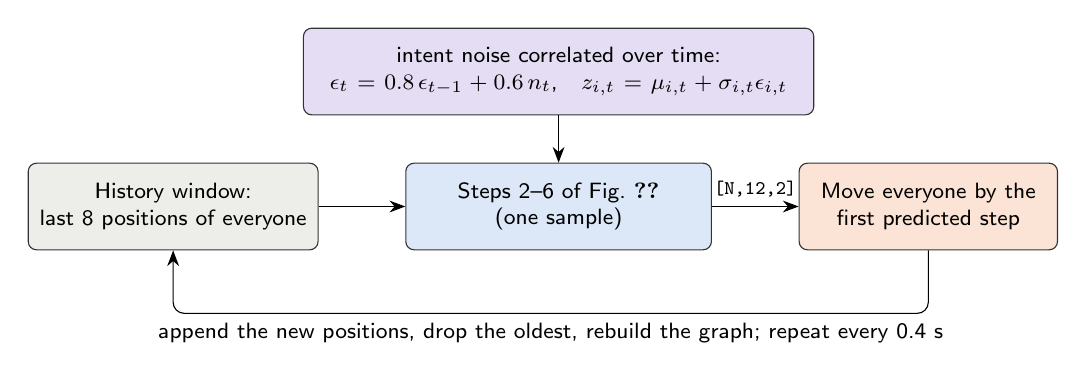
\begin{tikzpicture}[font=\sffamily\footnotesize, >={Stealth[length=2mm]},
  blk/.style={draw=ink, rounded corners=3pt, align=center, minimum height=11mm, inner sep=4pt}]
\node[blk, fill=inp, text width=34mm] (w) {History window:\\ last 8 positions of everyone};
\node[blk, fill=enc, right=11mm of w, text width=36mm] (f) {Steps 2--6 of Fig.~\ref{fig:overview}\\ (one sample)};
\node[blk, fill=lat, above=6mm of f, text width=62mm] (n) {intent noise correlated over time:\\ $\epsilon_t=0.8\,\epsilon_{t-1}+0.6\,n_t$,\quad $z_{i,t}=\mu_{i,t}+\sigma_{i,t}\epsilon_{i,t}$};
\node[blk, fill=dec, right=11mm of f, text width=30mm] (x) {Move everyone by the first predicted step};
\draw[->] (w) -- (f);
\draw[->] (n) -- (f);
\draw[->] (f) -- node[above, font=\ttfamily\scriptsize]{[N,12,2]} (x);
\draw[->, rounded corners] (x.south) -- ++(0,-8mm) -| node[pos=0.25, below]{append the new positions, drop the oldest, rebuild the graph; repeat every 0.4 s} (w.south);
\end{tikzpicture}
\caption{Closed loop. The correlated noise keeps each pedestrian's intent consistent while letting it change
slowly. Rollout fine-tuning \vb{R} trains through exactly this loop.}
\end{figure}

%%SNIP src/simplenavsim/realism/sim.py 200 250 Simulator loop%%

%======================================================================
\appendix
\section{Hyperparameters (read from the checkpoints)}
%======================================================================
\begin{tabularx}{\textwidth}{@{}l l X@{}}
\toprule
Component & Setting & Value \\
\midrule
Graph & neighbours / radius & 24 / 10 m (STEPS-only: 16) \\
Encoder & width / representation & 256 / 128; node and edge temporal layers 2 / 3; 4 heads; 2 graph rounds; dropout 0.09 \\
Decoder & width / intent & 512 / 64 (STEPS-only: 32); 1 social round; dropout 0.06 \\
Training & optimiser & AdamW, LR $3\times10^{-4}$, warm-up + cosine, weight decay 0.0022, grad clip 1.0, 60 epochs \\
& KL weight $\beta$ & 0.0799 (collision-aware: 0.15), 10-epoch warm-up \\
Collision-aware & refinement rounds / $\lambda_{\text{col}}$ / radius & 1 / 10 / 0.4 m \\
Rollout fine-tuning & LR / rollout length & $5\times10^{-5}$ / 4 $\to$ 12 steps; 300 batches of 2048 pedestrians per epoch \\
Simulator & intent noise correlation & $\rho=0.8$ \\
Selection & oversampling & 4 ($4K$ drawn, $K$ kept); group rule 1 m / 0.3 m/s \\
\bottomrule
\end{tabularx}

%======================================================================
\section{Evaluation metrics}
%======================================================================
\begin{itemize}
\item \textbf{Best-of-$K$ ADE/FDE (per pedestrian)}: for each pedestrian, the smallest average / final error over its $K$ samples.
\item \textbf{Scene-level best-of-$K$}: one sample index for the whole scene (the best one), then average over pedestrians.
\item \textbf{Single-sample ADE}: average error of a random sample; \textbf{mode ADE}: error of the $z=\mu$ prediction.
\item \textbf{Close-contact rate}: share of pedestrians within 0.2 m / 0.4 m of another at some predicted step, ignoring observed walking groups.
\item \textbf{Realism W1}: Wasserstein-1 distance between predicted and real distributions of speed, acceleration, turning rate and nearest-neighbour distance.
\end{itemize}

\end{document}
